%
%
\chapter{Funktionsprinzipien und Implementierungen} 
%
%
% Das Query-Modell von MyCoRe
%
%
\section{Das Query-Modell von MyCoRe}
%
%
MyCoRe bem�ht sich, das Synatx-Modell der Suchabfragen an die existierenden Standards des W3C f�r {\bf XML Path Language (XPath) Version 1.0} (W3C Recommendation 16 November 1999) und {\bf XQuery 1.0: An XML Query Language} (W3C Working Draft 22 August 2003) anzugleichen. Dabei muss aber auch R�cksicht auf die Spezifik des MyCoRe-Systems zur Suche von Objekten und Metadaten genommen werden. Daher ist MyCoRe nicht  100\% XPath/XQuery konform, es wird sich jedoch bem�ht, wo irgend m�glich die Spezifikationen einzuhalten. Grund f�r diese Abweichungen sind die Praxisorientierung des MyCoRe-Systems, vor allem im Bereich digitaler Bibliotheken. So sollen verschiedene Persistence-Systeme zum Einsatz kommen, welche sehr unterschiedliche Abfrage-Syntax, auch au�erhalb der XML-Welt, implementieren. Daher stellen der in diesem Abschnitt beschriebene Abfrage-Syntax nur einen recht keinen Teil der M�glichkeiten der W3C Spezifikationen dar. Er gen�gt aber in der Praxis, um recht komplexe Projekte zu realisieren.\\[2ex]
MyCoRe muss neben der eigentlichen Query noch erfahren, welche Datenmodell-Typen abzufragen sind. Auch daf�r ist die Ursache in der Persistence-Unabh�ngigkeit von MyCoRe zu suchen. Es ist notwendig, die Typen auf die entsprechenden Stores zu mappen, damit die Suche erfolgreich ist. Als Beispiel soll hier der Content Manager 8 ItemType oder die Umsetzung unter eXist stehen. M�glich ist sowohl einzelne Typen, wie auch eine Liste davon anzugeben. Die Liste ist ein String mit folgendem Syntax:
\begin{verbatim}
String type_list = "type1[,...]"
\end{verbatim}
Wichtig ist nur, dass die Elemente, nach denen gefragt wird, in allen Datenmodellen der Typen vorkommen (sonst k�nnte das Ergebnis der Suche falsch sein). Normalerweise wird die Typ-Liste in der Applikation festgelegt und an die entsprechenden Query-Schnittstellen im API �bergeben, z. B. durch das SearchMaskServlet.\\[2ex]
%
\subsection{Operatoren}
MyCoRe verwendet nur die folgenden Operatoren innerhalb eines Test. Dies begr�ndet sich mit der Kompatibilit�t und Umsetzung gegen�ber den einzelnen Persitence-Layern. Wenn weitere Operatoren ben�tigt werden, so m�ssen diese in ALLEN Persitence-Implementierungen eingebaut werden. \\[2ex]
Die einzelnen {\cc Test} k�nnen wiederum mit {\cc AND} bzw. {\cc OR} verkn�pft werden. Funktionen f�r Test werden unter MyCoRe NICHT unterst�tzt. 
\begin{verbatim}
SingleQuery :: OutPath [ Tests ]
               Tests
Tests       :: Test { AND | OR Test ... }
Test        :: InPath Operator Value
\end{verbatim}
\begin{itemize}
\item Operator = - ist f�r alle Values zul�ssig
\item Operator != - ist f�r alle Values zul�ssig
\item Operator < - ist nur f�r Datums- und Zahlenangaben zul�ssig
\item Operator <= - ist nur f�r Datums- und Zahlenangaben zul�ssig
\item Operator > - ist nur f�r Datums- und Zahlenangaben zul�ssig
\item Operator >= - ist nur f�r Datums- und Zahlenangaben zul�ssig
\item Operator like - versucht im Value den angegebenen String zu finden, als Wildcard ist * zul�ssig
\item Operator contains - arbeitet wie like, ist eine TextSearch-Engine verf�gbar, so erfolgt die linguistische Suche darin.
\end{itemize}
Die Operatoren {\bf like} und {\bf contains} sind eine Erg�nzung von MyCoRe um mit Textsuch-Mechanismen arbeiten zu k�nnen. Sie sind so nicht Bestandteil der W3C Spezifikationen, habe sich aber in der Praxis bewehrt.\\[2ex]
%
\subsection{Pfadangaben}
Die Pfadangaben f�r eine SingleQuery k�nnen einfach oder einmal geschachtelt sein, je nach dem, wie die einzelnen Text- bzw. Attributknoten des XML-Datenmodells logisch zusammengeh�ren. Alle hier aufgef�hrten M�glichkeiten sind relativ zu XML-Dokument-Wurzel.\\
\begin{verbatim}
OutPath :: a
           a/b
InPath  :: SpecialNodeFuncition
           @d
           text()
           c
           c/text()
           c/@d
           c/d/@e
           c/d/text()
SpecialNodeFuncition :: *
                        text()
                        doctext()
\end{verbatim}
Hier noch einige Hinweise:
\begin{itemize}
\item '*' als {\cc SpecialNodeFuncition} darf allein nur in einer {\cc SingleQuery} ohne {\cc OutPath} angegeben werden. Es erfolgt dann eine Suche �ber alle f�r TextSearch markierten Metadaten.
\item 'text()'  als {\cc SpecialNodeFuncition} darf allein nur in einer {\cc SingleQuery} ohne {\cc OutPath} angegeben werden. Es wird nach '*' �berf�hrt.
\item 'doctext()'  als {\cc SpecialNodeFuncition} ist f�r die Abfrage des TextSearch des Dokumentes vorgesehen.\footnote{Wird derzeit implementiert und ist bald verf�gbar!}
\item MyCoRe kann bei Bedarf der Applikation um weitere {\cc SpecialNodeFuncition}'s erg�nzt werden.
\end{itemize}
Nun einige g�ltige Beispiele :
\begin{verbatim}
text() contains "..."
* like "..."
@ID = "..."
metadata/rights/right = "..."
metadata/rights/right/text() = "..."
metadata/masse/mass[text() = "..." and @type = "..."]
doctext() contains "..."
\end{verbatim}
%
\subsection{Abfragen von Objekt-Metadaten}
Unter Objekt-Metadaten sind alle Datenmodell-Typen zu verstehen, welche NICHT {\bf class} oder {\bf derivate} sind\footnote{siehe auch UsersGuide, Abschnitt 3.2.3}. Alle XML-Files der Objekt-Metadaten Typen haben als Master-Tag {\bf /mycoreobject} und genau auf diesen Knoten als Return-Value zielen auch alle Queries unter MyCoRe. Der allgemeine Syntax ist also:
\begin{verbatim}
Query  :: OneQuery { AND|OR OneQuery { AND|OR ... } }
OneQuery :: /mycoreobject[ SpecialNodeFuncition ]
\end{verbatim}
Dies bedeutet, es k�nnen mehrere Abfragen hintereinander mit AND oder OR verkn�pft werden. F�r jedes Metadatum des Datenmodells ist eine {\cc OneQuery} zu formulieren. Das diese Anfragen alle auf den selben Datenraum laufen, daf�r sorgt die oben beschiebene Festlegung des Typ-Elementes. Somit erhalten Sie ein korrektes Gesamtergebnis.\\[2ex]
%
\subsection{Resultat der Query}
Alle Antworten als Resultat der Anfrage werden in einem XML-Conatiner zusammengefasst und der Anwendung zur�ckgegeben. Der Aufbau des Containers ist dabei Persitence-unabh�ngig. Nachfolgend die XML-Struktur des Resulates eine Query:
\lstset{language=XML,fancyvrb=true,frame=btlr,breaklines,prebreak={\space\MyHookSign}}
\begin{lstlisting}[caption=XML-Syntax eines Metadaten-Objektes,label=lst:xml_syntax_mcrresults]
<mcr_results parsedByLayoutServlet="...">
<mcr_result host="..." id="..." rank="0" hasPred="..." hasSucc="...">
<mycoreobject 
  ...
</mycoreobject>
</mcr_result>
</mcr_results>
\end{lstlisting}
Das Attribut \mcridentifier{parsedByLayoutServlet} ist ein Flag, welches eine etwaige Vorverarbeitung des Ergebnisses durch das LayoutServlet anzeigt.\\[2ex]
Das Attribut \mcridentifier{host} beinhaltet entwerden '{\bf local}' oder den den Hostalias des Servers, von dem das Resultat stammt.\\[2ex]
Das Attribut \mcridentifier{id} ist die entsprechende MCRObjectID des Resultates.\\[2ex]
Das Attribut \mcridentifier{hasPred} ???\\[2ex]
Das Attribut \mcridentifier{hasSucc} ???\\[2ex]
%
\subsection{Abfragen von Derivaten}
F�r die Derivate gelten die selben Regeln f�r die Queries. Bachten Sie jedoch, dass das Datenmodel fest vorgeschieben ist und das Master-Tag anders heisst. Das Resultat auf eine Anfrage wird auch in einen {\bf mcrresults}-Container verpackt.
\begin{verbatim}
Query  :: OneQuery { AND|OR OneQuery { AND|OR ... } }
OneQuery :: /mycorederivate[ SpecialNodeFuncition ]
\end{verbatim}
%
\subsection{Abfragen von Klassifikationen}
Klassifikationen werden in MyCoRe-Anwendungen erfahrungsgem�� am h�ufigsten abgefragt. Die Klassifikationen k�nnen nur nach einem sehr festen Schema abgefragt werden, wobei entwerder die gesamte Klassifikation oder nuer eine einzelne Kategorie zur�ckgegeben wird. Die XML-Struktur entspricht dabei immer der einer Klassifikation.
\begin{verbatim}
Query :: /mycoreclass[@ID = "..." { and @category like "..." } ]
\end{verbatim}
%
\subsection{Klassen�bersicht}


%
\section{Das Metadatenmodell}
\subsection{MCRClassification}
\subsection{MCRObject}
\subsection{MCRDerivate}
\subsection{MCRLinkManager}
\subsection{Erweiterungsm"oglichkeiten}
\section{Das IFS Modell (ohne Stores)}
%
\section{Die Benutzerverwaltung}

Dieser Teil der Dokumentation beschreibt Funktionalit"at, Design, Implementierung und 
Nutzung des MyCoRe Subsystems f"ur die Benutzerverwaltung. 

\subsection{Die Gesch"aftsprozesse der MyCoRe Benutzerverwaltung}
Das Benutzermanagement ist die Komponente von MyCoRe, in der die Verwaltung derjenigen 
Personen geregelt wird, die mit dem System umgehen (zum Beispiel als Autoren Dokumente 
einstellen). 
Zu dieser Verwaltung geh"ort auch die Organisation von Benutzern in Gruppen. 
Eine weitere Aufgabe dieser Komponente ist das Erm"oglichen einer Anmelde/-Abmeldeprozedur.

Ein Use-Case Diagramm (siehe Abbildung \ref{fig:UserUseCases} soll eine Reihe 
typischer Gesch"aftsprozesse des Systems zeigen (ohne dabei den Anspruch zu haben, alle 
Akteure zu benennen oder alle Assoziationen der Akteure mit den Gesch"aftsprozessen 
zu definieren).

\begin{figure}[h]
  \begin{center}
    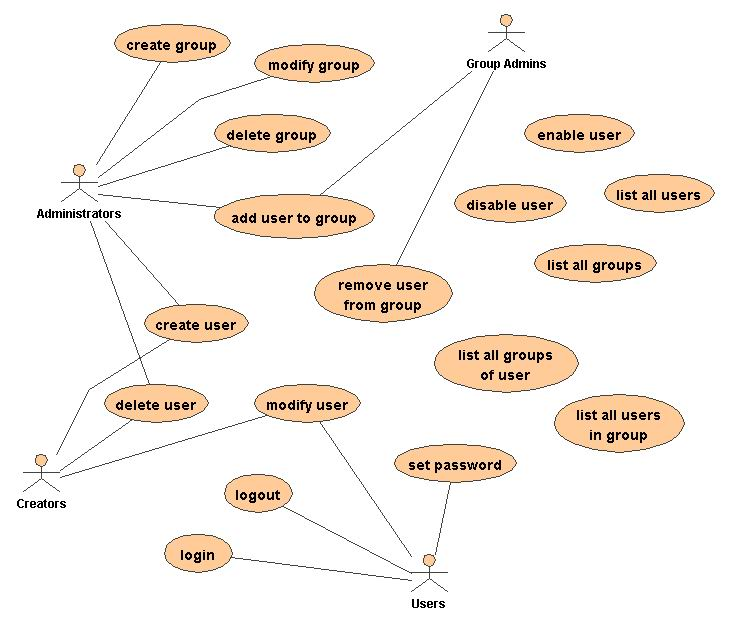
\includegraphics[scale=0.55]{ProgGuide_2User_UseCase.jpg}
    \caption{Gesch"aftsprozesse der Benutzerverwaltung in MyCoRe}
    \label{fig:UserUseCases}
  \end{center}
  \vspace{-1.4cm}
\end{figure} 

Offensichtlich d"urfen nicht alle Akteure des Systems die Berechtigung haben, alle 
Gesch"aftsprozesse durchf"uhren zu k"onnen. 
Daher muss ein System von Privilegien und Regeln implementiert werden: Benutzer/innen 
haben Privilegien (z.B. die Berechtigung, neue Benutzer/innen zu erstellen). 
Die Vergabe der Privilegien wird durch die Mitgliedschaft der Benutzer/innen in Gruppen 
geregelt. 
Dar"uber hinaus muss das System definierten Regeln gehorchen. 
So gen"ugt z.B. das Privileg "add user to group" allein nicht, 
um genau das Hinzuf"ugen eines Benutzers zu einer Gruppe definieren zu k"onnen. 
Die Regel ist in diesem Fall, dass ein Administrator jeden beliebigen Benutzer in 
jede beliebige Gruppe setzen kann, jeder andere Benutzer mit diesem Privileg aber maximal 
die Zugeh"origkeit zu Gruppen vergeben kann, in denen er or sie selbst Mitglied ist. 
Auf diese Weise wird verhindert, dass sich ein Benutzer oder eine Benutzerin selbst 
h"ohere Privilegien zuweisen kann. 
Die Privilegien und Regeln der MyCoRe-Benutzerverwaltung werden weiter unten ausf"uhrlich 
aufgef"uhrt.

\subsection{Benutzer, Gruppen, Privilegien und Regeln}
{\bf Benutzer}\\
Die Attribute von Benutzer/innen des Systems k"onnen in drei Bereiche klassifiziert 
werden, den account-Informationen wie ID, Passwort, Beschreibung usw., 
den Adress-Informationen wie Name, Anrede, Fakult"atszugeh"origkeit usw. sowie 
den Informationen "uber die Mitgliedschaft zu Gruppen. 
Die aktuell implementierten Benutzerattribute kann man an folgender beispielhafter 
XML-Darstellung erkennen:

{\bf to be continued ...}

%
\section{Zugriffsrechte und Access Control Lists}
\section{Der Backend-Store}
\subsection{DB2 / MySQL / Oracle}
% Das Backend f�r IBM Content Manager 8.2
%
%
\subsection{Das Backend f�r IBM Content Manager 8.2}
%
%
\subsubsection{Umsetzung der Queries}
%
{\bf Hinweise!} 
\begin{itemize}
\item Strings, welche NUR Zahlen enthalten, werden als Zahl interpretiert. L�uft die Anfrage gegen ein als 'VarChar' definiertes Attribut, kommt es zum Fehler  durch den CM. Erg�nzen Sie den Zahlen-String in der Suche z. B. mit einem '*' und benutzen Sie den Like Operator. Beispiel {\tt a like '0004*'}.
\end{itemize}

% Das Backend f�r XML:DB
%
%
\subsection{Das Backend f�r XML:DB}
%
%
\subsubsection{Umsetzung der Queries}
%
{\bf Hinweise!} 
\begin{itemize}
\item eXist ignoriert derzeit Schachtelungen eines Test mit '[...]'. Daher kann das Ergebnis der Anfrage mehr Treffer haben, als bei korrekter Ausf�hrung der Query.
\end{itemize}

\subsection{Filesystem-Store}
\subsection{VideoStores}
\subsection{RemoteStore im Detail}
\subsection{Weitere Ausbaum�glichkeiten}
%
\pagebreak
\section{Die Frontend Komponenten}
\label{sec:Frontend}

\subsection{Das Commandline-Tool und seine Erweiterungen}
\subsection{Das Zusammenspiel der Servlets mit dem MCRServlet}
\label{sec:CommonServlets}

Als "ubergeordnetes Servlet mit einigen grundlegenden Funktionalit"aten dient die 
Klasse MCRServlet.
Die Hauptaufgabe von MCRServlet ist dabei die Herstellung der Verbindung zur
Sessionverwaltung (siehe Abschnitt \ref{sec:Sessionverwaltung}).
Das Zusammenspiel der relevanten Klassen ist im folgenden Klassendiagramm 
(Abbildung \ref{fig:MCRServletClasses}) verdeutlicht.

\begin{figure}[h]
  \begin{center}
    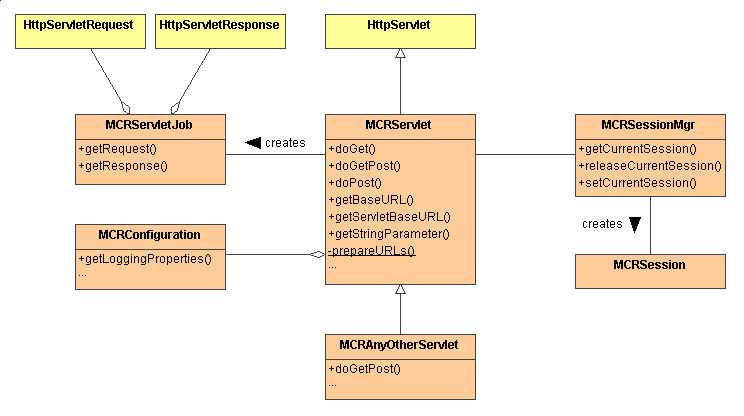
\includegraphics[scale=0.62]{ProgGuide_2Frontend_MCRServlet.jpg}
    \caption{Klassendiagramm Common Servlets}
    \label{fig:MCRServletClasses}
  \end{center}
  \vspace{-1.4cm}
\end{figure} 

Wie an anderen Stellen im MyCoRe-System auch, kann auf Konfigurationsparameter wie
zum Beispiel den Einstellungen f"ur das Logging "uber das statische Attribut
MCRConfiguration zugegriffen werden.
Dies wird ausf"uhrlich in Kapitel \ref{sec:Konfiguration} beschrieben.

MCRServlet selbst ist direkt von HttpServlet abgeleitet.
Sollen andere Servlets im MyCoRe Softwaresystem die von MCRServlet angebotenen 
Funktionen automatisch nutzen, so m"ussen sie von MCRServlet abgeleitet werden.
Im Klassendiagramm ist das durch die stellvertretende Klasse MCRAnyOtherServlet
angedeutet.
Es wird empfohlen, dass die abgeleiteten Servlets die Methoden doGet() und doPost() 
nicht "uberschreiben, denn dadurch werden bei einem eingehenden Request auf jeden 
Fall die Methoden von MCRServlet ausgef"uhrt.

Der Programmablauf innerhalb von MCRServlet ist im folgenden Sequenzdiagramm 
(Abbildung \ref{fig:MCRServletSequenz}) dargestellt.
Bei einem eingehenden Request (doGet() oder doPost()) wird zun"achst an 
MVRServlet.doGetPost() delegiert.
%
\footnote{Bei dieser Delegation wird ein Parameter mitgef"uhrt, "uber den feststellbar 
          ist, ob es sich um einen GET- oder POST-Request gehandelt hat.}

\begin{figure}[h]
  \begin{center}
    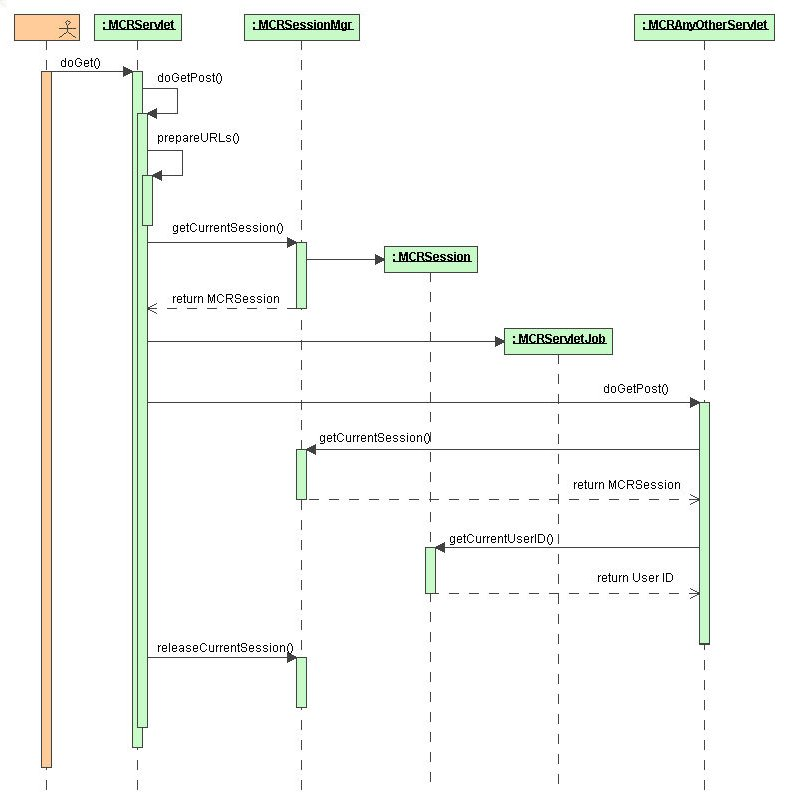
\includegraphics[scale=0.52]{ProgGuide_2Frontend_MCRServletSequenz.jpg}
    \caption{Sequenzdiagramm Common Servlets}
    \label{fig:MCRServletSequenz}
  \end{center}
  \vspace{-1.4cm}
\end{figure} 

Falls nicht schon aus vorhergehenden Anfragen an das MCRServlet bekannt, werden 
in doGetPost() die Base-URL und die Servlet-URL des Systems bestimmt. 
Dabei besteht die Servlet-URL aus der Base-URL und dem angeh"angten String 'servlets/'.
Darauf folgend wird die f�r diese Session zugeh"orige Instanz von MCRSession
bestimmt.
Das Verfahren dazu ist im Ablaufdiagramm \ref{fig:MCRServletFluss} dargestellt. 

\begin{figure}[h]
  \begin{center}
    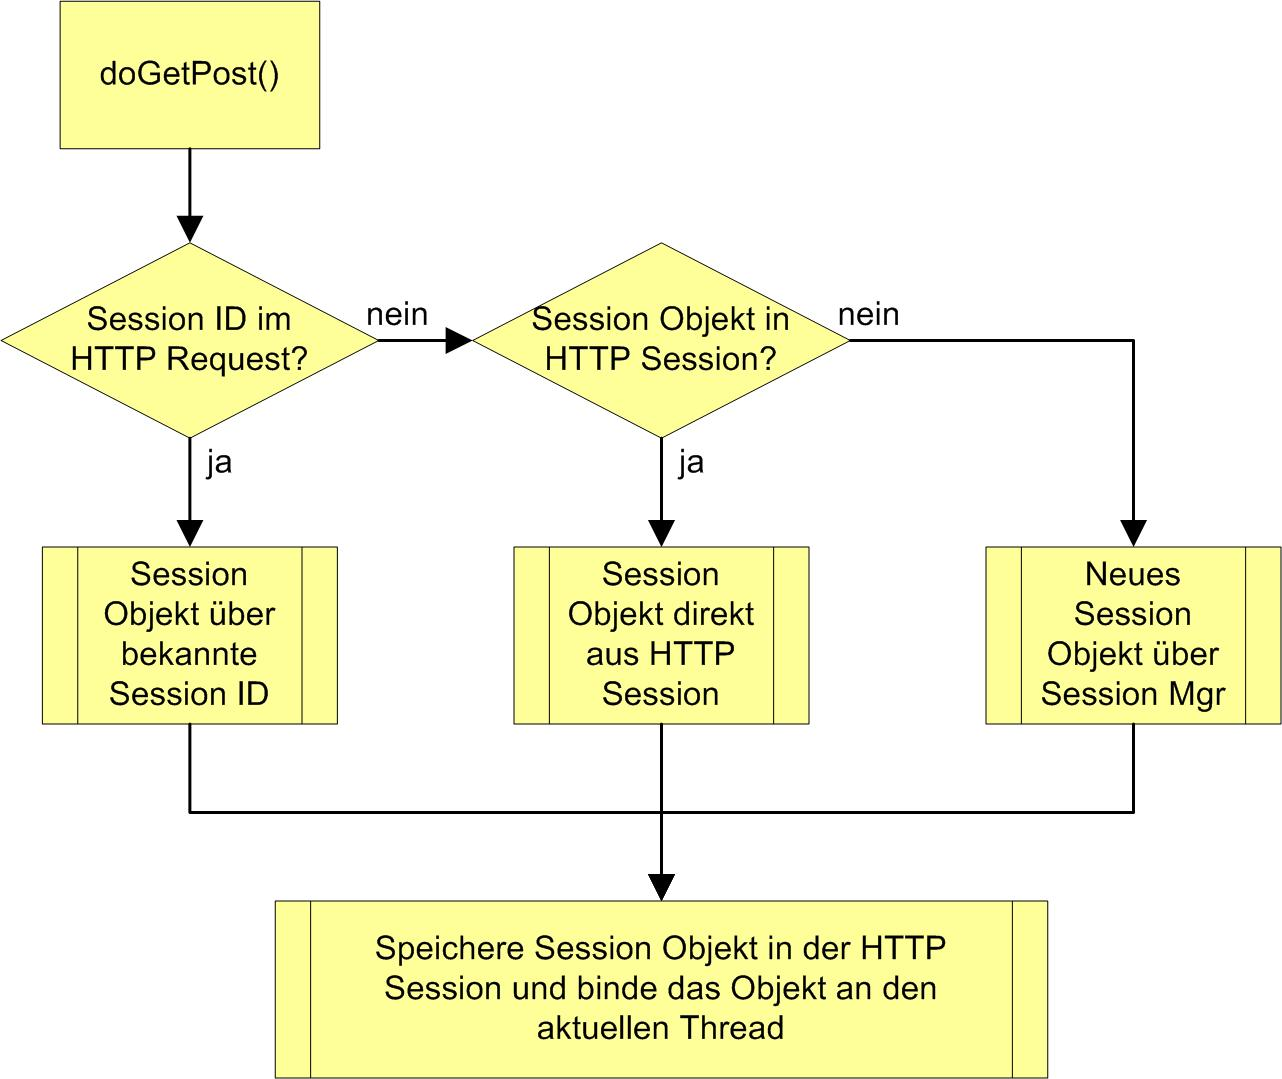
\includegraphics[scale=0.35]{ProgGuide_2Frontend_MCRServletFluss.jpg}
    \caption{Ablaufdiagramm f"ur MCRServlet.doGetPost()}
    \label{fig:MCRServletFluss}
  \end{center}
  \vspace{-1.4cm}
\end{figure} 

Die Session kann bereits durch vorhergehende Anfragen existieren. 
Falls dies der Fall ist, kann das zugeh"orige Session-Objekt entweder "uber eine im 
HttpServletRequest mitgef"uhrte Session ID identifiziert oder direkt der HttpSession
entnommen werden.
Existiert noch keine Session, so wird ein neues Session-Objekt "uber den Aufruf von
MCR\-Session\-Mgr.\-get\-Current\-Session() erzeugt (vergleiche Abschnitt \ref{sec:Sessionverwaltung}).
Nachfolgend wird das Session-Objekt an den aktuellen Thread gebunden und zus"atzlich in der
HttpSession abgelegt.
%
\footnote{Das Speichern des Session-Objekts in der Http-Session ist notwendig, weil in 
          einer typischen Servlet-Engine mit Thread-Pool Umgebung nicht davon ausgegangen 
          werden darf, dass bei aufeinanderfolgenden Anfragen aus demselben Kontext auch 
          derselbe Thread zugeweisen wird. Siehe auch Abschnitt \ref{sec:Sessionverwaltung}.}

Im Sequenzdiagramm \ref{fig:MCRServletSequenz} gehen wir davon aus, dass die Sitzung neu ist
und deswegen ein Session-Objekt "uber MCRSessionMgr.getCurrentSession() erzeugt werden muss.
Schliesslich wird eine Instanz von MCRServletJob erzeugt.
Diese Klasse ist nichts weiter als ein Container f"ur die aktuellen HttpServletRequest- und 
HttpServletResponse Objekte und hat keine weitere Funktionalit"at (siehe Klassendiagramm
\ref{fig:MCRServletClasses}).

An dieser Stelle wird der Programmfluss an das abgeleitete Servlet (in diesem 
Beispiel MCRAnyOtherServlet) delegiert.
Dazu muss das Servlet eine Methode mit der Signatur

{\tt public void doGetPost(MCRServletJob job) \{\}}

implementieren. 
Wie das Sequenzdiagramm \ref{fig:MCRServletSequenz} beispielhaft zeigt, kann 
MCRAnyOtherServlet danach gegebenenfalls auf das Session-Objekt und damit auf die
Kontextinformationen zugreifen.
Der Aufruf an den Session Manager dazu w"are:

{\tt MCRSession mcrSession = MCRSessionMgr.getCurrentSession();}

Es sei bemerkt, dass dies nicht notwendigerweise genau so durchgef"uhrt werden muss.
Da wegen den geschilderten Problemen mit thread-local Variablen in Servlet-Umgebungen
das Session-Objekt auch in der Http-Session abgelegt sein muss, k"onnte man die
Kontextinformationen auch aus der "ubergebenen Instanz von MCRServletJob gewinnen.


\subsection{Das Login-Servlet und MCRSession}

Das Login-Servlet, implementiert durch die Klasse MCRLoginServlet, dient zum 
Anmelden von Benutzern und Benutzerinnen "uber ein Web-Formular.
Die Funktionsweise ist wie folgt:
Wie in Abschnitt \ref{sec:CommonServlets} empfohlen, "uberschreibt MCRLoginServlet 
nicht die von MCRServlet geerbten Standard-Methoden doGet() und doPost().
Meldet sich ein Benutzer oder eine Benutzerin "uber das MCRLoginServlet an, so wird
daher zun"achst die Funktionalit"at von MCRServlet ausgenutzt und die in Abschnitt 
\ref{sec:CommonServlets} beschriebene Verbindung zur Sessionverwaltung herstellt.
Wie dort ebenfalls beschrieben, wird der Programmfluss an das Login-Servlet "uber
die Methode MCRLoginServlet.doGetPost() delegiert.
Der Ablauf in doGetPost() wird im folgenden Diagramm (Abbildung 
\ref{fig:MCRLoginServletFluss}) dargestellt und ist selbsterkl"arend.

\begin{figure}[h]
  \begin{center}
    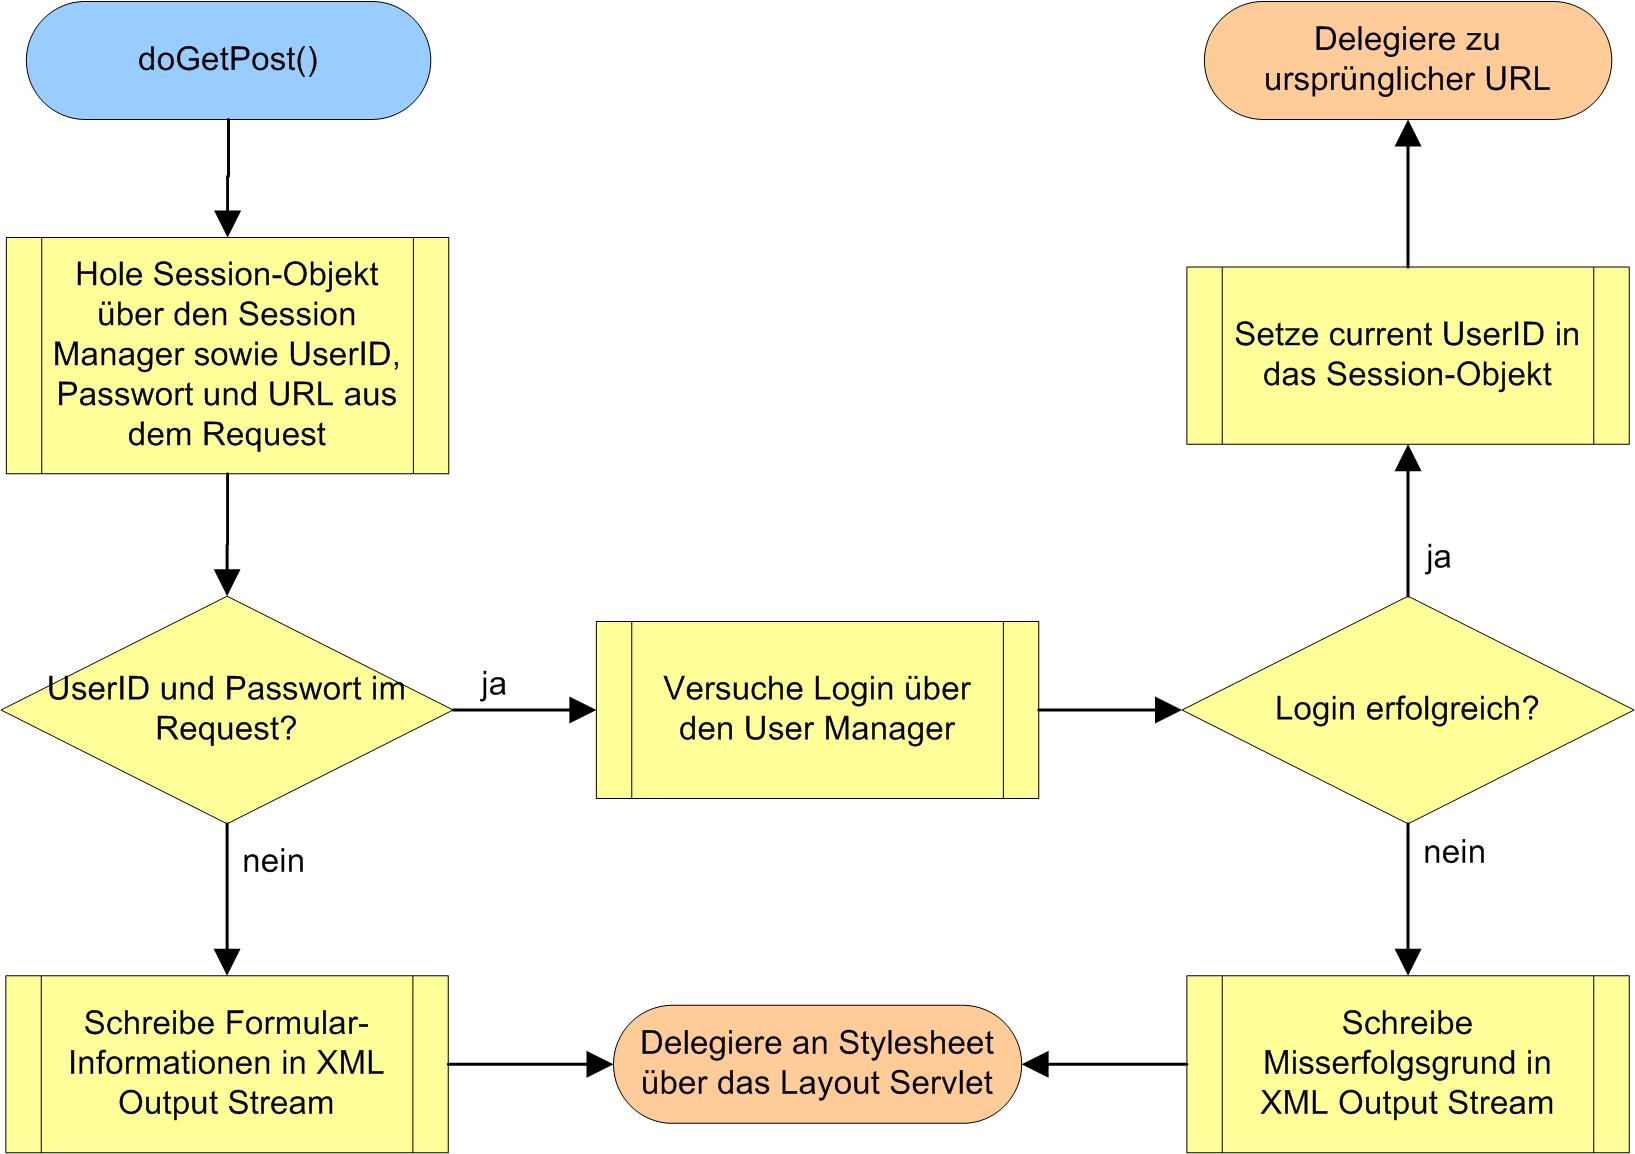
\includegraphics[scale=0.35]{ProgGuide_2Frontend_MCRLoginServletFluss.jpg}
    \caption{Ablaufdiagramm f"ur MCRLoginServlet.doGetPost()}
    \label{fig:MCRLoginServletFluss}
  \end{center}
  \vspace{-1.4cm}
\end{figure} 

Der resultierende XML Output-Stream muss vom zugeh"origen Stylesheet verarbeitet
werden und hat die folgende Syntax:

\vspace{0.5cm}
\lstset{language=XML, fancyvrb=true, frame=btlr, breaklines, prebreak={\space\McrHookSign}}
\begin{lstlisting}[caption={[XML Output des Login Servlets]XML Output des Login Servlets},%
                  captionpos=b, label=lst:XmlLoginServlet, frame=lines]
<mcr_user unknown_user="true|false"
          user_disabled="true|false"
          invalid_password="true|false">
  <guest_id>...</guest_id>
  <guest_pwd>...</guest_pwd>
  <url>...<url>
</mcr_user>
\end{lstlisting}

Bei einer missgl"uckten Anmeldung wird der Grund daf"ur in Form eines Attributes
auf true oder false gesetzt.
Das Stylesheet kann dann die entsprechende Meldung ausgeben.
Die Gast-User ID und das Gast-Passwort werden aus einer Konfigurationsdatei gelesen.
Die URL schlie"slich wird dem Http-Request entnommen und sollte dort von der
aufrufenden Seite bzw. vom aufrufenden Servlet gesetzt sein.
Ist sie nicht gesetzt, so wird die Base-URL des MyCoRe-Systems verwendet.

\subsection{IFS-Servlet}
\subsection{Query-Servlet}
\subsection{Innere Struktur des Editor-Servlets}
\subsection{Innere Struktur des User-Servlets}

%
\section{Funktionsprinzipien der Services}
\subsection{OAI}
\subsection{NBN}
\subsection{Weitere}
